\documentclass[conference]{IEEEtran}
\IEEEoverridecommandlockouts
% The preceding line is only needed to identify funding in the first footnote. If that is unneeded, please comment it out.
%Template version as of 6/27/2024

\usepackage{cite}
\usepackage[T1]{fontenc}
\usepackage{amsmath,amssymb,booktabs,multirow,xcolor,url,tabularx,array}
\usepackage{graphicx}
\usepackage[hidelinks]{hyperref}
\usepackage{xcolor}
\def\BibTeX{{\rm B\kern-.05em{\sc i\kern-.025em b}\kern-.08em
    T\kern-.1667em\lower.7ex\hbox{E}\kern-.125emX}}
\begin{document}

\title{[Experiment, Analysis, and Benchmark] Evaluating Language Models and Subspace Methods for Explaining Known Tabular Outliers}

\author{
\IEEEauthorblockN{Lili Guan\IEEEauthorrefmark{1},~Lei Duan\IEEEauthorrefmark{2},~Weiyan Zhang\IEEEauthorrefmark{1},~Xinye Wang\IEEEauthorrefmark{3}, ~Hengmin Zhang\IEEEauthorrefmark{4},~Tong Ruan$\boxtimes$\IEEEauthorrefmark{1}}
%\IEEEauthorrefmark{1}\IEEEauthorrefmark{4}}
\IEEEauthorblockA{\IEEEauthorrefmark{1}
School of Information Science and Engineering, East China University of Science and Technology, Shanghai, China}
\IEEEauthorblockA{\IEEEauthorrefmark{2}
School of Artificial Intelligence, Sichuan University, Chengdu, China}
\IEEEauthorblockA{\IEEEauthorrefmark{3}
School of Artificial Intelligence, Tiangong University, Tianjin, China}
\IEEEauthorblockA{\IEEEauthorrefmark{4}
State Key Laboratory of Industrial Control Technology, East China University of Science and Technology, Shanghai, China}
\IEEEauthorblockA{\{guanlili, weiyanzhang, zhanghengmin, ruantong\}@ecust.edu.cn, leiduan@scu.edu.cn, wangxinye@tiangong.edu.cn}
}

\maketitle

\begin{abstract}
Explaining a flagged table row requires deciding which fields jointly distinguish it from normal data. Row labels and injected edits do not determine this explanation: a modified field can be ordinary alone, and several irreducible combinations can be valid. We present a benchmark that completely enumerates population-minimal support explanations, separates them from rule and edit targets, and audits the evidence available in finite references. A unified comparison gives three language models and subspace methods the same candidate information and budget, with fixed structured output for the models. It also includes direct enumeration of sample-minimal explanations. On 96 paired targets, Qwen reaches exact recovery of 0.385 and Gower-LOF 0.646; the enumeration baseline reveals a separate gap between candidate coverage and first-choice ranking. Complete-population, new-rule, invoice, and public expert-decision workloads expose different failure modes. Invoices show how duplicate-sensitive density ratios compete across discrete projections: treating distinct-coordinate neighborhoods raises LOF recovery from 0.000 to 0.229, while changing the numerical floor does not improve it. Public correction records provide a separate inspection target. These results show how label semantics, available evidence, and method configuration determine anomaly-explanation comparisons.
\end{abstract}
\begin{IEEEkeywords}
data quality, anomaly explanation, feature subspaces, large language models, benchmark evaluation
\end{IEEEkeywords}

\section{Introduction}
Investigating a data-quality alert requires choosing fields to inspect. A value can be ordinary alone and unusual in combination with other attributes. In \emph{known-outlier explanation}, a method receives a flagged row, its schema, and finite normal references, then returns ranked field subsets. The upstream detector score and the target's clean counterpart are unavailable~\cite{li2024xadsurvey}. The evaluation must specify what makes one of those subsets a correct explanation. Fig.~\ref{fig:intro-real} shows an archived Pima query and peer agreement~\cite{han2022adbench}.

\textbf{One invoice, different targets.} Consider net $25$, tax $1$, and gross $14$ (Fig.~\ref{fig:framework}). The clean domain permits net $\in\{10,15,20,25\}$, tax $\in\{0,\ldots,4\}$, and gross $=\text{net}+\text{tax}$. The recorded edit changes gross, yet $(10,4,14)$ is normal, so gross alone has normal support. Both \{net, gross\} and \{tax, gross\} are minimal exclusions; their union is redundant. Recovering the edit and recovering a minimal explanation therefore give different answers.

\begin{figure}[t]
\centering
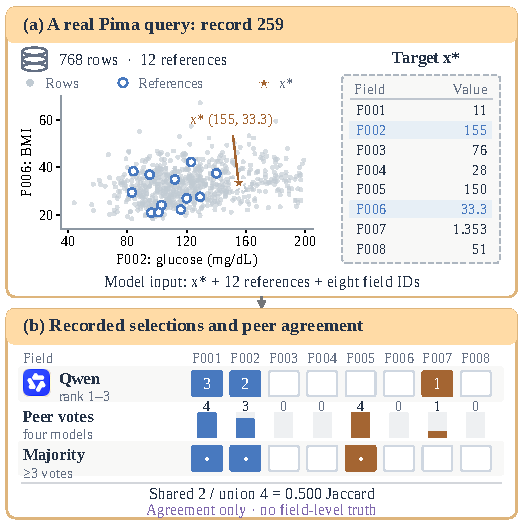
\includegraphics[width=\columnwidth]{figures/figure_intro_real_dataset.pdf}
\caption{Pima query C0035 (row 259): 752 nonzero glucose/BMI pairs, 12 reference rings, and the target star. Cells align Qwen ranks with the four-peer majority; bars show votes. Brown marks disagreement. Models receive opaque IDs; Jaccard measures agreement without field-level truth.}
\label{fig:intro-real}
\end{figure}

\begin{figure*}[t]
\centering
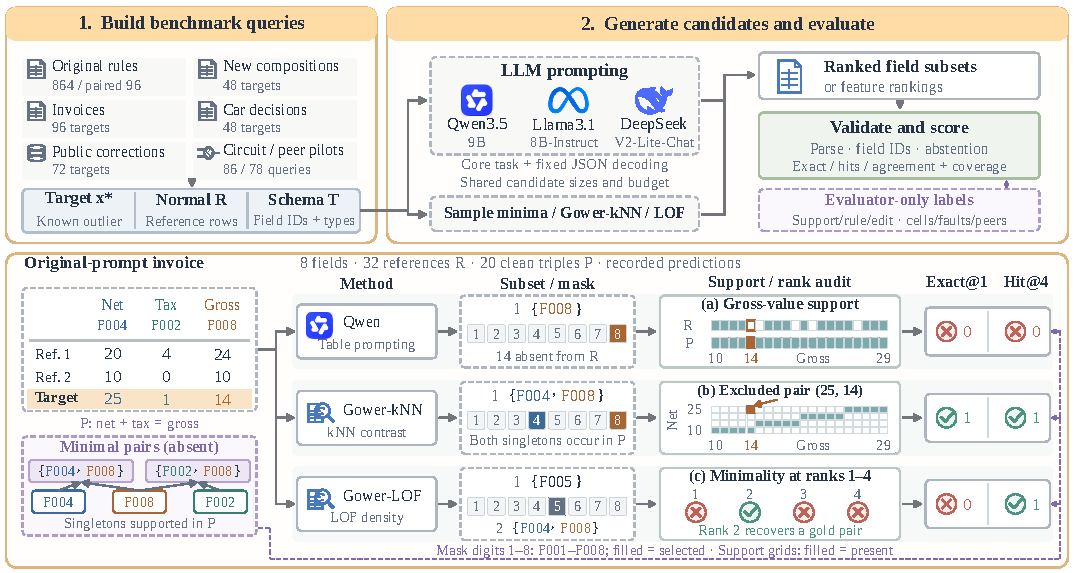
\includegraphics[width=\textwidth]{figures/figure2_overall_framework.pdf}
\caption{Evaluation framework and recorded invoice \texttt{constraint\_tax\_total\_000}. The overview shows the unified core task; auxiliary tracks retain their own configurations and labels. The lower trace preserves outputs from the original prompt, illustrating why candidate generation and support verification differ. It displays three of eight fields and two of 32 references. Gross 14 is absent from $R$ but present in the 20-triple population $P$; the net--gross pair is excluded; LOF's second candidate is minimal. Purple paths carry evaluator-only information.}
\label{fig:framework}
\end{figure*}

\textbf{Why compare language models?} A prompt can describe mixed field types, serialize examples, and request candidate subsets without fitting a separate model to every schema. LLM-based data-quality systems such as ZeroED and ZeroEC generate criteria, labels, or correction rules from context~\cite{ni2025zeroed,wu2025zeroec}. Table-anomaly and cleaning benchmarks similarly motivate evaluating this interface~\cite{choudhury2025tabard,gu2025radar,li2025autodcworkflow}. Here, three fixed models must infer useful combinations from the supplied rows. Opaque or neutral names restrict the main comparison to that evidence; the experiment does not establish performance for larger models, tool-using systems, or domain-rich prompts.

\textbf{The evaluation problem.} Relevant-subspace evaluation already allows multiple correct subsets and exact set matching~\cite{myrtakis2021comparative}. The unresolved issue addressed here is how to define \emph{all} minimal explanations of a population, distinguish those labels from an edit history, and assess methods that see only a sample. A projection absent from the references may occur elsewhere in the normal population. Conversely, a model may return a supported or redundant set even when every normal row is visible. Candidate size information and output requirements can further change a method comparison.

\textbf{Our approach.} We enumerate complete clean populations and their inclusion-minimal support exclusions, separating rule and provenance labels. The original 864 cases span 38 templates. The unified comparison shares targets, references, size information, and four-candidate budgets, with fixed JSON output for LLMs and a direct sample-enumeration baseline. New rules, invoice constraints, and an independent expert table extend the comparison (Fig.~\ref{fig:framework}).

The study asks: \textbf{RQ1: Labels.} How do population support, rules, and recorded changes alter evaluation? \textbf{RQ2: Evidence and configuration.} How do references, candidate priors, and output contracts affect a common-task comparison? \textbf{RQ3: Scoring mechanisms.} Which implementation choices contribute to cross-workload ranking reversals?

Our contributions are:
\begin{itemize}
\item \textbf{Complete population-minimal labels and evidence audits.} We distinguish support, rule, mechanism, and edit targets. Sample and population minimal-set families disagree in 862 of 864 original cases; this measures family disagreement, not non-identifiability. Deterministic proxies change support and rule labels in 211 cases.
\item \textbf{A unified comparison with a direct support baseline.} Shared candidate information and fixed structured output enter the same experiments. Sample enumeration separates finding plausible candidates from ranking them, while repeated references and complete populations diagnose available evidence.
\item \textbf{A mechanism analysis of discrete subspace ranking.} Matched invoice experiments isolate numerical floors, boundary ties, and duplicate handling. Public corrections and expert decisions clarify which conclusions transfer under unchanged explanation semantics and which concern a different target.
\end{itemize}



\section{Task and Label Semantics}

Given schema $T$ with fields $F=\{f_1,\ldots,f_d\}$, known outlier $x^*$, and normal references $R$, a method returns ranked subsets
\[
\widehat{\mathcal E}(x^*,R,T)=(S_1,\ldots,S_K),\qquad S_k\subseteq F,
\]
optionally with evidence, confidence, or abstention.

Let $P_X$ denote the clean population and $\pi_S$ the projection onto $S$. A subset is \emph{support-sufficient} when $\pi_S(x^*)$ has no match in $P_X$. It is \emph{rule-sufficient} when every full domain assignment matching $x^*$ on $S$ satisfies the anomaly predicate. A sufficient subset is inclusion-minimal when no proper subset is sufficient. We retain the complete minimal families $\mathcal S_{\mathrm{support}}^{\min}$ and $\mathcal S_{\mathrm{rule}}^{\min}$; inclusion-minimal sets can differ in size. Separate provenance labels record directly edited fields $M_{\mathrm{direct}}$, all value changes $M_{\mathrm{value}}$ including propagation, and fields capable of affecting the anomaly rule $M_{\mathrm{rule}}$.

\textbf{When support and rule labels coincide.} Let $\mathcal D$ be the disclosed Cartesian domain and $A$ the anomaly predicate. If $P_X=\{x\in\mathcal D:\neg A(x)\}$, absence of a clean completion is equivalent to every completion satisfying $A$. The two minimal families then coincide. Additional clean-population constraints can break this equivalence: a deterministic proxy can exclude clean completions without appearing in $A$. Section V-A gives an observed example.

For $A(f_1)\lor B(f_2)$ with both terms true, either singleton can be minimal, whereas their union is redundant. Our primary label is population-minimal descriptive support; Table~\ref{tab:semantics} separates it from unobserved edit provenance.

A population-absent projection is absent from $R$, but sampling can create additional absences. We keep population labels fixed and audit sample-minimal alternatives separately.

\textbf{Checking an explanation.} For a clean row $r$, let $D(r)=\{f_j:r_j\ne x^*_j\}$ contain the fields on which it differs from the target. Then support sufficiency is equivalent to
\[
  S\cap D(r)\ne\varnothing\quad\text{for every }r\in P_X.
\]
Each normal row must therefore be distinguished by at least one selected field. To check minimality, remove each field $f$ from $S$ in turn. A minimal set has a normal witness matching $x^*$ on $S\setminus\{f\}$ for every such removal. These witnesses show why every selected field is necessary. Checking single-field removals suffices because absence is preserved when more fields are added. Replacing $P_X$ by $R$ gives the sample criterion, which has fewer rows to distinguish and can admit additional explanations.

For the invoice in Fig.~\ref{fig:framework}, gross 14 occurs with net 10 and tax 4, and net 25 occurs with other gross values. Both singletons thus have normal witnesses, whereas the pair $(25,14)$ has none. A large candidate containing this pair is sufficient but need not be minimal. This distinction also explains why a feature ranking alone cannot certify an explanation: its prefix length and the joint support of the selected values determine whether the candidate meets the task definition.

\begin{table}[t]
\centering
\caption{Label semantics and identification from an unpaired query with finite normal references and no hidden generator.}
\begin{tabularx}{\columnwidth}{|l|>{\raggedright\arraybackslash}X|>{\raggedright\arraybackslash}p{1.65cm}|}
\hline
Label & Meaning and inferability & Use \\
\hline
Support & Minimal absent projections; finite references need not identify them & Primary \\
Rule & Minimal subsets forcing anomaly; hidden predicate required & Alternative \\
Mechanism & Fields affecting anomaly; hidden rule required & Relevance \\
Direct edit & Recorded edits; hidden intervention history required & Provenance \\
Value change & Changes including propagation; paired clean row required & Provenance \\
Corrected field & Published dirty/clean difference; source convention required & Inspection \\
Peer agreement & Overlap with other model selections; no field truth & Agreement \\
\hline
\end{tabularx}
\label{tab:semantics}
\end{table}



\section{Benchmark Construction}
\subsection{Procedural support benchmark}

Each of three seeds generates 40 templates with 12 cases each, split into eight training, eight development, and 24 test templates. The 864 test cases cover 38 templates. Splits are disjoint within each seed but overlap across seeds. Earlier results informed this reevaluation; bootstrap and multiplicity correction cannot remove that selection bias. New-composition validation freezes methods before generating different rules.

Eight families cover numeric marginals, categorical rarity, pairs, conditional groups, multiple valid sets, edit/mechanism differences, relational comparisons, and higher-order logic. Each seed tests three of five templates per family; pooled family summaries involve four or five templates and remain descriptive.

Cases contain 6/12/24 fields and 8/16/32 references, with finite numeric, ordinal, binary, categorical, date-like, and identifier-like domains. Marginal factors are balanced; joint cells are not. Six nuisance profiles cover independent noise, a 64-category distractor, noisy and deterministic proxies, a pre-edit frozen proxy, and independent categorical missingness. Dates and identifiers are distractors. Complete profiles and joint case/template counts are in the artifact.

The generator enumerates clean/anomalous role assignments, samples a hidden clean row and target, binds roles to random IDs, and adds distractors and references. Sufficient subsets are enumerated with deterministic proxy constraints, then nonminimal sets are removed. Independent distractors are marginalized. Changing individual roles checks rule relevance; direct and propagated changes are recorded separately. Rule IDs, logic, clean rows, and labels are withheld.

An independent seeded permutation then determines schema, target, and reference column order, preserving values, labels, and field-name bindings. Identity permutations are allowed. Half the cases expose random neutral names. Separate display seeds prevent the role-binding prefix from becoming a fixed cue.




The primary paired panel consists of all 96 first-split test targets with 32 references, four per template. Its selection is independent of method outputs. This panel supports a controlled comparison on 24 original templates, not an independent replacement for the original test distribution.

\subsection{Standards-derived invoice constraints}

An independent finite-domain workload instantiates four Peppol billing relations~\cite{peppol2026billing}: line net equals quantity times unit price plus charges minus allowances (R120, base quantity one); document net equals summed line nets plus charges minus allowances (BR-CO-13); gross equals net plus tax (BR-CO-15); and amount due equals gross minus paid plus rounding (BR-CO-16). These are synthetic integer amounts, not collected invoices or a full conformance test.

The four normal relations contain 144, 144, 20, and 48 structured rows. We change one field to another value in its clean marginal, retaining 24 distinct invalid targets per relation before inference. Each query has eight opaque fields, independent categorical distractors, 32 clean references, and independently ordered columns. Exhaustive population checks enumerate all support minima, marginalizing distractors. Support and rule labels coincide because the anomaly predicate complements the normal relation; direct edits remain separate. The original prompt is diagnostic; the unified comparison follows Section IV. Both Gower methods search all 255 nonempty subsets. Scores average the four relations equally.



\subsection{New compositions and complete evidence}

We freeze the checkpoints, original prompt, parser, and decoding before generating four invalid targets for each of 12 new Boolean compositions. The six-field rules use four to six essential coordinates, exceeding the original maximum of three. Parity, disjoint conjunctions, conditional parity, multiplexer, count-balance, and majority-consistency rules have distinct 64-row truth tables. Fixed-seed target selection precedes inference. Gower searches all 63 subsets; all methods have four answers.

Each target receives an independent 32-row sample with replacement. The first two targets per rule additionally receive two samples and the complete normal population, yielding 24 matched targets and 120 inputs per method. Complete evidence includes every normal tuple and declares completeness in the prompt; these changes are inseparable. The rules were designed after review, not externally curated as blind tasks. Model and protocol choices were not adjusted to their results.

Scores average targets within rules, then the 12 rules equally. Strata use minimum truth size (1--2, 3, 4--6), alternative count (1, 2--4, $\geq5$), and extra sample minima (0, 1--3, $\geq4$). Repeated samples fix the target, schema, display, and population labels; they are not independent tasks.


The unified configuration is fixed before its new generations on these existing queries. We retain the original full-prompt results as diagnostics; the joint rerun does not make this previously examined workload a fresh blind test.

\subsection{Independent expert decision table}
UCI Car Evaluation~\cite{bohanec1988car} is derived from an expert decision model and completely covers its six-attribute categorical domain. We verify that the 1,728 distinct rows equal the Cartesian product of the published domains. The 518 configurations labeled acceptable, good, or very good define $P_X$; an unacceptable configuration is the flagged target. Exhaustive projection checks produce the same population-minimal support labels as in Section II. This supplies an independent source of normal constraints, with no injected edit serving as explanation truth.

Before inference, a fixed seed selects 12 unacceptable targets per buying-price category. Each of the 48 queries receives 32 acceptable references without replacement. Random opaque IDs and independently shuffled columns preserve values. Selection strata, source labels, rules, and populations are hidden; all 63 nonempty subsets are eligible. This is one expert decision system, not observed anomaly incidents; opaque IDs cannot exclude pretraining exposure.

\subsection{Auxiliary targets}
\textbf{Public corrections.} Flights, Beers, and Rayyan dirty/clean pairs from Raha and Baran supply 72 queries~\cite{mahdavi2019raha,mahdavi2020baran}. Each source contributes eight targets with one, two, or at least three corrections, selected before predictions. Each query has 32 corrected references excluding held-out targets; Flights also excludes the same flight. Raw strings and source identities are retained; index fields are removed. Hidden clean counterparts identify acceptable singleton inspection targets, including formatting changes, not minimal support explanations.

\textbf{Circuits and peer agreement.} Sixteen table pairs from four gate-negation circuits yield 64 targets and 86 focus-output queries, with 16 references each. Their fault input sets contain 1--12 fields; 47 exceed three. The artifact verifies changed-output alignment over 66,834 anomalous rows~\cite{antwarg2024groundtruth}. A separate five-model pilot covers 70 ADBench queries and eight UCI Lymphography queries~\cite{han2022adbench}. UCI uses two source-class-1 normal rows, whereas ADBench uses its binary labels and 142 normal rows. Circuit fault recovery and peer agreement retain their own denominators and are never pooled with support accuracy.

\section{Evaluation Protocol}
\subsection{Unified core configuration}
The primary comparison includes Qwen3.5-9B, DeepSeek-V2-Lite-Chat, Llama-3.1-8B-Instruct, sample-minimal enumeration (SME), Gower-kNN, and Gower-LOF. All receive the same target, schema, normal rows, and field order. The LLMs return only ranked feature subsets and an abstention flag. They are explicitly told the same size cap used by search: three fields on the paired panel, six on new rules and Car decisions, and eight on invoices. Every method has a budget of four distinct nonempty subsets. No field identities or hidden labels accompany the size information.

The three checkpoints use the existing shared loader and chat templates, greedy batch-one decoding, a 16,384-token input limit without truncation, and 512 output tokens. A fixed JSON-schema token filter enforces the core object, legal IDs, four candidates, and the relevant size cap~\cite{lmfe2026}. The original parser rejects repeated IDs; repeated candidate sets collapse in their existing order. An oversized or empty set invalidates an answer, without truncating or reranking fields. Abstention suppresses attached candidates. Invalid, missing, input-rejected, and abstained queries remain recovery failures.

The configuration is frozen before 1,080 new model queries: 360 per checkpoint across the paired panel, 120 new-rule conditions, 96 invoices, and 48 Car targets. It follows earlier-result inspection, not preregistration. Checkpoints, prompts, and decoding are evaluated together. The core contract excludes auxiliary classification, mechanisms, evidence sentences, and confidence.

\subsection{Direct sample-minimal enumeration}
SME enumerates nonempty field sets within the shared cap using only visible rows. It retains a set if the target projection is absent and each single-field removal restores support. Candidates are sorted by cardinality, then canonical feature-ID tuple; the first four are returned. This fixed ranking uses no hidden labels or learned relevance. Canonical IDs make ties independent of display order, without claiming optimal ranking.

Full-family size and population-label retention distinguish candidate availability from ranking. With complete normal evidence and an unrestricted candidate space, SME must return population minima for any target outside the population. Finite references can instead create small spurious candidates that rank before valid explanations.

\subsection{Statistical rankers and original adapters}
\textbf{Gower rankers.} Gower distance averages reference-range-scaled differences for numeric, ordinal, and date-like fields and mismatch distances for categorical, binary, and identifier fields~\cite{gower1971similarity}. Missing-value mismatches score one. Exhaustive search uses the same candidate caps as the LLMs and SME. Gower-kNN ranks the target's three-neighbor mean distance relative to the median and dispersion of reference leave-one-out distances. Gower-LOF uses reference-only local reachability densities~\cite{breunig2000lof}. The target never enters the fitted reference graph. Score ties are resolved by subset size and canonical IDs. The existing ranker predictions are reproduced exactly on all 312 previously evaluated query conditions per method.

\textbf{Original diagnostic suite.} The 864-case comparison retains its original full LLM contract and unequal size prior: Gower knew that all population minima had at most three fields, while the model prompt did not. Table~\ref{tab:original} is therefore secondary to the unified comparison. Controls include all fields, the first three display positions, a univariate rarity/deviation ranking, and random subsets whose size distribution is estimated from training labels over 100 random seeds. SME is added under the same three-field cap.

SOD, COP, and M\textsuperscript{2}OE use legal-domain scaling, one-hot categorical encoding, and explicit missing coordinates~\cite{kriegel2009sod,angiulli2024m2oe}. Their outputs are task adaptations: SOD selects a low-variance subspace, COP maps local-PCA errors to fields, and M\textsuperscript{2}OE supplies both field choices and repair masks. M\textsuperscript{2}OE's unordered choices use a separate three-choice endpoint. The RLAX adaptation uses a reference-distance PPO reward with 256 interactions and four epochs, with 1,024/4,096-interaction development diagnostics~\cite{amirato2026rlax}. Beam retains 100 pairs before expanding to triples; a matching exhaustive pair/triple search isolates pruning~\cite{myrtakis2021comparative}. We make no convergence or speed claims for these adapters.

\subsection{Metrics, aggregation, and uncertainty}
Support Exact@1 and Hit@4 are the primary endpoints. For ranked candidates $(S_1,\ldots,S_K)$ and the complete minimal family $\mathcal G$,
\begin{align}
\mathrm{Exact@1}&=\mathbb I[S_1\in\mathcal G],\\
\mathrm{Hit@4}&=\mathbb I[\exists k\leq4:S_k\in\mathcal G],\\
\mathrm{Suff@1}&=\mathbb I[\exists G\in\mathcal G:G\subseteq S_1].
\end{align}
Sufficiency, best-set Jaccard, rule scores, candidate size, and validity remain secondary. An answer requires a valid, non-abstaining, nonempty candidate list. The all-query denominator is retained; conditional size and quality use answered queries only. Duplicate sets add no credit.

Aggregation units are 24 templates for paired targets, 12 rules for new compositions, four relations for invoices, and 48 cases from one source for Car. Cases are averaged within each unit before equal-unit averaging. The original estimator averages seed--template cells, then seeds within templates, then 38 templates. No cross-track accuracy is computed.

Tables report mean $\pm$ sample SD across the declared units. SD describes between-unit heterogeneity, not repeated-model-run variation or uncertainty of the mean. Paired-panel contrasts additionally use 2,000 template-bootstrap replicates. Archived sign-flip diagnostics assume null symmetry of template differences and apply Holm correction within their declared endpoint families; they cannot remove bias from repeated inspection of original templates. New transfer tasks, parameter sweeps, and source strata are descriptive. The artifact retains original intervals and all per-case scores.

\subsection{Configuration and evidence diagnostics}
Original diagnostics vary the size instruction, output contract, structured decoding, output length, field order, and reference quantity. The full contract additionally requests task labels, mechanisms, evidence, and confidence; removing these changes the task beyond formatting. Historical conditions explain the unified design but do not form a factorial causal estimate. Four random displays and nested 8/16/32 references preserve targets and labels; role-aware front/back displays are oracle diagnostics.

For the same 24 new-rule targets, three independent 32-row draws are compared with the complete normal population. The complete condition also declares completeness to the model. Its effect therefore combines coverage with that declaration. Error categories distinguish unavailable answers, valid minima, nonminimal population exclusions, sample-only exclusions, and projections already supported by visible rows. The categories describe observable errors; they do not establish a universal reasoning-error rate or an information-theoretic recovery bound.

\subsection{LOF and correction-source diagnostics}
Invoice controls preserve the same 96 targets and references while varying candidate size, neighbor count, numerical floor, tie selection, and duplicate treatment. The new floor sweep uses $10^{-6}$, $10^{-9}$, and $10^{-12}$ with $k=3$. Fixed-$k$ choices use the original selection routine or canonical ascending/descending reference order for distance ties. Inclusive neighborhoods contain every reference within the $k$-distance boundary, with numerical equality tolerance $10^{-12}$. We also collapse identical projections before inclusive-neighbor scoring, and separately use a radius reaching three distinct non-identical coordinates while retaining original multiplicities. If fewer distinct coordinates exist, the radius uses those available. These are explicit variants, not silent replacements for the original adapter.

The public-correction task requests four singleton suggestions; FieldHit@$k$ measures whether any of the first $k$ fields was changed in the supplied clean record. The original structured singleton protocol is retained unchanged. A post-hoc source audit separates quantity/null/location normalizations with explicit row-local certificates from time changes and source-specific bibliographic conventions. The absence of such a certificate does not prove that references are uninformative. We also rescore the same 16 multi-correction Beers queries after excluding ounces from the acceptable target set, without changing predictions.

\section{Labels, Evidence, and Unified Comparisons}
\subsection{RQ1: What changes when the explanation label changes?}
Support and rule families coincide in 653 of 864 original cases. All 211 differences involve deterministic proxies. On those cases, changing only the scoring label reduces original Qwen Exact@1 from 0.275 to 0.137 and Gower-LOF from 0.487 to 0.191. Thus, part of an apparent performance difference can arise from which explanatory object the evaluator accepts.

In one deterministic-proxy case, the rule requires $F011>0.5$ and $F007\in\{c4,c5\}$, while F008 copies F007. The rule minimum is \{F007,F011\}; support also accepts \{F008,F011\}. The target has $F011=1$ and $F007=F008=c4$. An edit to F007 propagates to F008. Rule scoring rejects the proxy alternative, whereas evaluating all changed fields rewards a redundant set. Fig.~\ref{fig:framework} supplies the complementary invoice example: every target has one edited field, but its valid support minima contain at least two fields. Multiple valid answers and exact set matching are established evaluation ideas; the additional requirement here is complete population enumeration with explicit rule and provenance separation.

\subsection{RQ2: Jointly controlling the primary comparison}
\begin{table*}[t]
\centering
\caption{Unified support comparison, mean $\pm$ SD. Paired targets use 24 template means, new rules 12 rule means, invoices four relation means, and Car 48 cases from one source. Shared size caps and four-candidate budgets apply within each track; all LLMs use fixed JSON decoding. Failures remain misses. Bold and underlining mark the highest and second-highest means; ties share marks.}
\begin{tabular}{|l|l|rrrrrr|}
\hline
Workload & Metric & Qwen & DeepSeek & Llama & SME & Gower-kNN & Gower-LOF \\
\hline
\multirow{2}{*}{\shortstack[l]{Paired targets\\(96; cap 3)}} & Exact@1 & $0.385\pm0.383$ & $0.031\pm0.084$ & $0.042\pm0.095$ & $0.313\pm0.348$ & $\underline{0.594\pm0.429}$ & $\textbf{0.646}\pm\textbf{0.396}$ \\
 & Hit@4 & $0.510\pm0.372$ & $0.042\pm0.095$ & $0.052\pm0.104$ & $0.646\pm0.403$ & $\underline{0.667\pm0.373}$ & $\textbf{0.719}\pm\textbf{0.378}$ \\
\hline
\multirow{2}{*}{\shortstack[l]{New rules\\(48; cap 6)}} & Exact@1 & $0.104\pm0.225$ & $0.042\pm0.097$ & $0.042\pm0.097$ & $\textbf{0.667}\pm\textbf{0.456}$ & $\underline{0.625\pm0.446}$ & $0.542\pm0.424$ \\
 & Hit@4 & $0.313\pm0.304$ & $0.042\pm0.097$ & $0.146\pm0.225$ & $\underline{0.813\pm0.322}$ & $\textbf{0.833}\pm\textbf{0.343}$ & $0.729\pm0.445$ \\
\hline
\multirow{2}{*}{\shortstack[l]{Invoices\\(96; cap 8)}} & Exact@1 & $0.010\pm0.021$ & $0.010\pm0.021$ & $0.031\pm0.040$ & $\underline{0.167\pm0.090}$ & $\textbf{0.406}\pm\textbf{0.191}$ & $0.000\pm0.000$ \\
 & Hit@4 & $0.208\pm0.068$ & $0.010\pm0.021$ & $0.073\pm0.052$ & $\underline{0.427\pm0.277}$ & $\textbf{0.510}\pm\textbf{0.138}$ & $0.115\pm0.129$ \\
\hline
\multirow{2}{*}{\shortstack[l]{Car decisions\\(48; cap 6)}} & Exact@1 & $0.479\pm0.505$ & $0.063\pm0.245$ & $0.083\pm0.279$ & $\textbf{0.958}\pm\textbf{0.202}$ & $0.896\pm0.309$ & $\underline{0.917\pm0.279}$ \\
 & Hit@4 & $0.625\pm0.489$ & $0.104\pm0.309$ & $0.083\pm0.279$ & $\textbf{0.979}\pm\textbf{0.144}$ & $0.896\pm0.309$ & $\underline{0.938\pm0.245}$ \\
\hline
\end{tabular}
\label{tab:unified}
\end{table*}
Table~\ref{tab:unified} jointly controls candidate information, four-candidate budgets, the core task, and structured output across the four support workloads. Qwen reaches Exact@1/Hit@4 of 0.385/0.510, compared with 0.646/0.719 for Gower-LOF and 0.594/0.667 for kNN. DeepSeek and Llama reach Exact@1 of 0.031 and 0.042. The ordering is observed directly under the joint configuration; it is not inferred from separate prior and formatting interventions.

Qwen's Exact@1 difference from LOF is -0.260, with a template-bootstrap interval [-0.344, -0.177], conditional on these 24 templates and frozen queries. Model coverage is 0.979/0.542/1.000. Input-cap failures and abstentions remain misses; common-feasible sensitivities are archived. The comparison concerns these fixed configurations, not general LLM capability.

\textbf{Finding candidates versus ranking them.} SME obtains Exact@1/Hit@4 of 0.313/0.646: greater top-four coverage than Qwen, but fewer correct first choices. Its family averages 96.604 candidates per query and retains 0.911 of population labels under equal-template weighting. This separates exposing valid alternatives from ranking them using size and IDs alone.

\subsection{Finite evidence and the direct support baseline}
The sample and population minimal-set families disagree in 862/864 cases, all with extra sample minima. This family-disagreement rate neither proves non-identifiability nor bounds any method's error. Equal-template means are 60.935 extra candidates and 0.863 population-minimum retention. SME obtains Exact@1/Hit@4 of 0.232/0.549.

The audit searches 41/298/2,324 subsets for 6/12/24 fields. Population-absent sets remain absent as references are added. A population minimum becomes sample-minimal when every proper subset has a matching witness; nested additions preserve its retention. Extra-minimum counts need not decrease: removing a spurious smaller minimum can expose several larger candidates. Retention and candidate counts thus capture different evidence limitations.

Under the original prompt, Qwen's first choice is sample-absent with frequency 0.873 but population-minimal with frequency 0.231; the remaining fractions are 0.336 population-insufficient and 0.306 sufficient but nonminimal. LOF's corresponding values are 0.734/0.514/0.197/0.024. These are classifications of outputs, not identified causes of individual failures. Difficulty strata in the artifact preserve truth size, number of valid alternatives, and extra sample minima; the dimensions co-vary with rule family and field count.

\subsection{Transfer under the same core configuration}
\begin{figure*}[t]
\centering
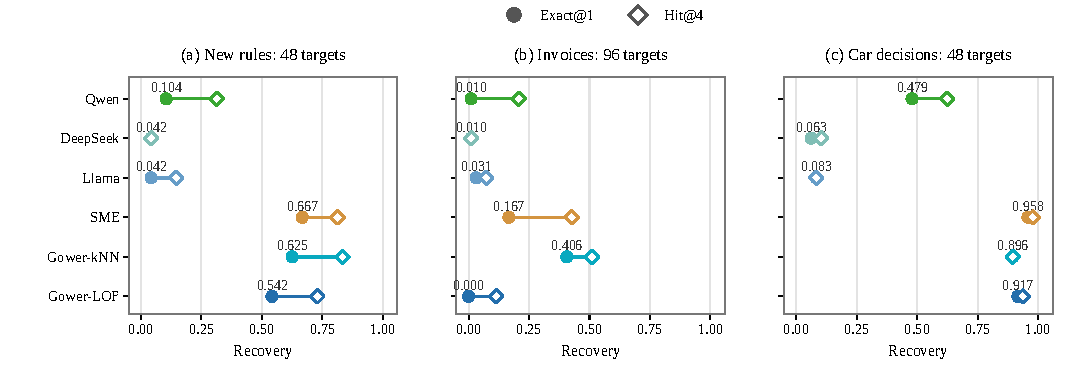
\includegraphics[width=\textwidth]{figures/figure_unified_transfer.pdf}
\caption{Unified support-localization configuration across three workloads. Filled circles show Exact@1 (annotated); open diamonds show Hit@4. New rules average 12 rule means, invoices four relation means, and Car decisions 48 targets from one source. SME is sample-minimal enumeration. All-query denominators and track-specific candidate caps are shared; these descriptive scores are not pooled.}
\label{fig:transfer}
\end{figure*}

Fig.~\ref{fig:transfer} compares the three transfer workloads under the unified configuration (Table~\ref{tab:unified}). On new rules, SME exceeds both Gower rankers at Exact@1. Sixteen targets require four- to six-field minima; full strata are archived. Original full-prompt Qwen reaches 0.167 versus the joint configuration's 0.104, so those results remain separate.

On invoices, kNN exceeds SME and the three models, while LOF reaches Exact@1 of 0.000. Eight queries admit a four-field alternative, and five have only four-field minima, motivating the full 255-candidate search. Section VI investigates the reversal on these fixed queries.

\textbf{Independent source with the same label semantics.} Car retains population-minimal support truth, unlike correction and circuit transfer. SME reaches Exact@1/Hit@4 of 0.958/0.979 (Table~\ref{tab:unified}). Of 48 targets, 43 admit a singleton minimum. On the five multi-field targets, SME/Qwen/kNN/LOF reach Exact@1 of 0.600/0.000/0.000/0.200. Simple exclusions and the single expert source limit wider conclusions.

\subsection{Repeated references and complete populations}
\begin{table*}[t]
\centering
\caption{Unified new-rule evidence diagnostics, mean $\pm$ SD across 12 rules. The three draws and Complete use the same 24 targets. Complete also declares exhaustive normal evidence. Stable counts targets with an answered, nonempty and identical first set across all three draws. Bold and underlined values are the largest and second-largest in each column; ties share marks.}
\begin{tabular*}{\textwidth}{@{\extracolsep{\fill}}|l|rr|rrr|rr|r|}
\hline
Method & \multicolumn{2}{c|}{New targets (48)} & \multicolumn{3}{c|}{Repeated references (same 24)} & \multicolumn{2}{c|}{Complete population (24)} & Stable \\
\cline{2-8}
 & Exact@1 & Hit@4 & Draw 1 Exact & Draw 2 Exact & Draw 3 Exact & Exact@1 & Hit@4 & / 24 \\
\hline
Qwen & $0.104\pm0.225$ & $0.313\pm0.304$ & $0.125\pm0.311$ & $0.000\pm0.000$ & $0.083\pm0.195$ & $0.208\pm0.334$ & $0.375\pm0.433$ & 1 \\
DeepSeek & $0.042\pm0.097$ & $0.042\pm0.097$ & $0.000\pm0.000$ & $0.000\pm0.000$ & $0.042\pm0.144$ & $0.000\pm0.000$ & $0.000\pm0.000$ & 8 \\
Llama & $0.042\pm0.097$ & $0.146\pm0.225$ & $0.042\pm0.144$ & $0.125\pm0.226$ & $0.042\pm0.144$ & $0.083\pm0.195$ & $0.125\pm0.226$ & 0 \\
\hline
SME & $\textbf{0.667}\pm\textbf{0.456}$ & $\underline{0.813\pm0.322}$ & $\textbf{0.708}\pm\textbf{0.450}$ & $\textbf{0.625}\pm\textbf{0.377}$ & $\textbf{0.708}\pm\textbf{0.396}$ & $\textbf{1.000}\pm\textbf{0.000}$ & $\textbf{1.000}\pm\textbf{0.000}$ & $\underline{11}$ \\
Gower-kNN & $\underline{0.625\pm0.446}$ & $\textbf{0.833}\pm\textbf{0.343}$ & $\underline{0.583\pm0.469}$ & $\underline{0.583\pm0.515}$ & $\underline{0.583\pm0.469}$ & $\underline{0.625\pm0.483}$ & $\underline{0.833\pm0.389}$ & 10 \\
Gower-LOF & $0.542\pm0.424$ & $0.729\pm0.445$ & $0.542\pm0.498$ & $0.542\pm0.498$ & $0.458\pm0.450$ & $0.583\pm0.515$ & $\underline{0.833\pm0.389}$ & $\textbf{12}$ \\
\hline
\end{tabular*}
\label{tab:unified-evidence}
\end{table*}

\begin{figure*}[t]
\centering
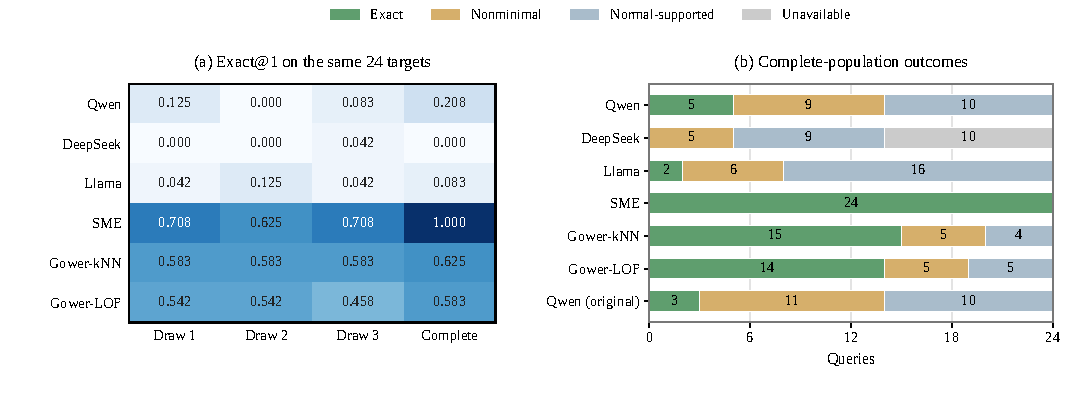
\includegraphics[width=\textwidth]{figures/figure_unified_evidence.pdf}
\caption{Evidence diagnosis on the same 24 targets from 12 new rules. (a) Exact@1 under three reference draws and complete normal evidence; hatches distinguish conditions. (b) Complete-population error counts; the last column retains original-prompt Qwen for comparison. Completeness also changes the prompt declaration. Sample-only exclusions are impossible in this condition.}
\label{fig:evidence}
\end{figure*}

SME recovers valid minima on all 24 complete-population queries (Fig.~\ref{fig:evidence}), making this finite task solvable from visible evidence. kNN and LOF reach Exact@1 of 0.625 and 0.583: removing sample ambiguity does not make novelty-score ranking optimize minimal support.

Joint Qwen obtains 5 exact answers, 9 nonminimal exclusions, 10 supported sets, and no unavailable answers under complete evidence. Original full-prompt Qwen produced 3/11/10/0; these are separate partitions. Missing references therefore cannot explain all errors in these settings, although the intervention combines additional rows with a completeness declaration.

Table~\ref{tab:unified-evidence} reports all draws and rule-level SDs. Extra sample minima average 1.542/1.208/1.000 across the three finite draws; complete evidence removes them. The archive records candidate retention and error types. Stability differs from accuracy: a repeated wrong set is stable, while switching between valid minima need not be an error.

\subsection{How the output contract changes the comparison}
\begin{figure}[t]
\centering
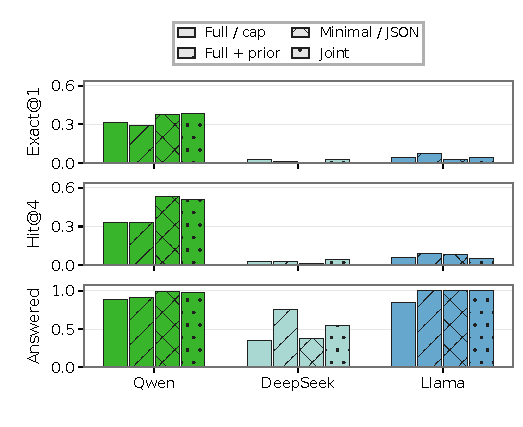
\includegraphics[width=\columnwidth]{figures/figure_unified_contract.pdf}
\caption{Configuration diagnostics on the same 96 targets. Full/cap applies the common size rule to original responses; Full+prior also states it. Minimal/JSON has constrained decoding without the three-field prior. Joint combines the core task, size information, and constrained output. Method colors and condition hatches follow the original plots. Answered reports valid non-abstaining coverage. The conditions do not isolate individual factorial effects.}
\label{fig:contract}
\end{figure}

The original shared-prior experiment changes Qwen/DeepSeek/Llama Exact@1 from 0.313/0.031/0.042 to 0.292/0.010/0.073 under the same size-enforced scoring. No paired change passes its six-test Holm correction. This addresses that instruction within the original full contract; it cannot predict the joint configuration by itself.

The reduced unconstrained prompt produced 94 similarly malformed Qwen JSON objects among 95 actual generations, each missing a candidate-object closing brace, despite a valid example. None exhausted 512 output tokens. Fixed-schema decoding on that same minimal prompt raises Qwen Exact@1 from 0.000 to 0.375 and Hit@4 from 0.010 to 0.531. Llama's validity reaches 1.000 but its Exact@1 remains 0.031; DeepSeek's nine output-cap failures and abstentions still limit usable answers. The joint configuration in Table~\ref{tab:unified} incorporates reliable output structure and shared size information in the same run.

The original non-answer bound, $\mathrm{Exact@1}+1-\mathrm{Answered}$, gives 0.239/0.292/0.211 for Qwen/DeepSeek/Llama, below LOF's original 0.514. This calculation holds existing answers fixed. It cannot bound an intervention that changes the content of already answered queries, as the contract experiments demonstrate.

\subsection{Original suite and adapter behavior}
\begin{table*}[t]
\centering
\caption{Original 864-case diagnostic: mean $\pm$ SD across 38 templates; answered-only size uses coverage-weighted template SD. Gower uses a three-field prior absent from the original LLM prompt. This table preserves the original configuration; Table~\ref{tab:unified} gives the joint comparison. Bold and underlining mark the highest and second-highest means across both panels, including controls; top-one fraction describes size, not quality. M\textsuperscript{2}OE is assessed separately.}
\begin{tabular}{|l|rrrrrr|}
\hline
Metric & \multicolumn{3}{c|}{LMs} & \multicolumn{3}{c|}{Rankers} \\
\hline
Metric & \shortstack{Qwen\\3.5-9B} & \shortstack{DeepSeek-V2\\Lite-Chat} & \shortstack{Llama-3.1\\8B-Instruct} & \shortstack{Gower\\LOF} & \shortstack{Gower\\kNN} & \shortstack{RLAX\\adaptation} \\
\hline
Support Suff.@1 & $0.537\pm0.300$ & $0.291\pm0.145$ & $0.183\pm0.161$ & $0.538\pm0.366$ & $0.608\pm0.330$ & $0.498\pm0.407$ \\
Support Exact@1 & $0.231\pm0.215$ & $0.023\pm0.037$ & $0.032\pm0.043$ & $\textbf{0.514}\pm\textbf{0.360}$ & $0.411\pm0.302$ & $\underline{0.426\pm0.384}$ \\
Support Hit@4 & $0.249\pm0.210$ & $0.039\pm0.051$ & $0.049\pm0.059$ & $\textbf{0.637}\pm\textbf{0.328}$ & $\underline{0.499\pm0.284}$ & $0.478\pm0.367$ \\
Support Jaccard@4 & $0.460\pm0.168$ & $0.200\pm0.052$ & $0.216\pm0.066$ & $\textbf{0.762}\pm\textbf{0.206}$ & $\underline{0.683\pm0.187}$ & $0.665\pm0.243$ \\
\hline
Rule Exact@1 & $0.202\pm0.198$ & $0.020\pm0.036$ & $0.024\pm0.032$ & $\textbf{0.451}\pm\textbf{0.340}$ & $0.351\pm0.289$ & $\underline{0.393\pm0.359}$ \\
Rule Hit@4 & $0.235\pm0.218$ & $0.032\pm0.050$ & $0.041\pm0.050$ & $\textbf{0.603}\pm\textbf{0.358}$ & $\underline{0.480\pm0.303}$ & $0.440\pm0.354$ \\
\hline
Top-one fraction & $0.228\pm0.065$ & $0.406\pm0.089$ & $0.202\pm0.013$ & $0.131\pm0.032$ & $0.197\pm0.053$ & $0.143\pm0.041$ \\
Answered & $\underline{0.992\pm0.019}$ & $0.731\pm0.087$ & $0.821\pm0.102$ & $\textbf{1.000}\pm\textbf{0.000}$ & $\textbf{1.000}\pm\textbf{0.000}$ & $\textbf{1.000}\pm\textbf{0.000}$ \\
\hline
Metric & \multicolumn{2}{c|}{Adaptations} & \multicolumn{4}{c|}{Controls} \\
\hline
Metric & \shortstack{SOD\\adaptation} & \shortstack{COP\\adaptation} & \shortstack{Univariate\\top four} & \shortstack{Random\\size prior} & All fields & \shortstack{First three\\positions} \\
\hline
Support Suff.@1 & $\underline{0.610\pm0.438}$ & $0.011\pm0.028$ & $0.144\pm0.207$ & $0.108\pm0.084$ & $\textbf{1.000}\pm\textbf{0.000}$ & $0.220\pm0.139$ \\
Support Exact@1 & $0.000\pm0.000$ & $0.011\pm0.028$ & $0.144\pm0.207$ & $0.033\pm0.021$ & $0.000\pm0.000$ & $0.002\pm0.014$ \\
Support Hit@4 & $0.000\pm0.000$ & $0.021\pm0.035$ & $0.391\pm0.406$ & $0.123\pm0.076$ & $0.000\pm0.000$ & $0.002\pm0.014$ \\
Support Jaccard@4 & $0.162\pm0.102$ & $0.144\pm0.071$ & $0.537\pm0.281$ & $0.343\pm0.018$ & $0.157\pm0.066$ & $0.154\pm0.056$ \\
\hline
Rule Exact@1 & $0.000\pm0.000$ & $0.009\pm0.022$ & $0.129\pm0.188$ & $0.028\pm0.019$ & $0.000\pm0.000$ & $0.002\pm0.014$ \\
Rule Hit@4 & $0.000\pm0.000$ & $0.018\pm0.030$ & $0.386\pm0.402$ & $0.106\pm0.072$ & $0.000\pm0.000$ & $0.002\pm0.014$ \\
\hline
Top-one fraction & $\underline{0.577\pm0.087}$ & $0.097\pm0.000$ & $0.097\pm0.000$ & $0.162\pm0.002$ & $\textbf{1.000}\pm\textbf{0.000}$ & $0.292\pm0.000$ \\
Answered & $\textbf{1.000}\pm\textbf{0.000}$ & $\textbf{1.000}\pm\textbf{0.000}$ & $\textbf{1.000}\pm\textbf{0.000}$ & $\textbf{1.000}\pm\textbf{0.000}$ & $\textbf{1.000}\pm\textbf{0.000}$ & $\textbf{1.000}\pm\textbf{0.000}$ \\
\hline
\end{tabular}
\label{tab:original}
\end{table*}
The original suite illustrates why sufficiency alone is inadequate. Qwen/LOF have Suff@1 of 0.537/0.538 but Exact@1 of 0.231/0.514; no equivalence is claimed. SOD reaches Suff@1 0.610 with zero exact recovery and selected-field fraction 0.577. Its objectives and unequal size prior distinguish this diagnostic suite from the unified ranking.

Native controls contextualize adapted scores. M\textsuperscript{2}OE's continuous repository example recovers all three injected fields in 7/10 seeds at 30 epochs: precision/recall 1.000/0.900 and mean distance reduction outside the clean cube 0.827. At 300 epochs these become exact recovery 0, recall 0.600, and reduction 0.375. SOD includes all three shifted low-variance coordinates in 20/20 cases but adds fields (precision 0.389). Native behavior validates neither mixed-type support adaptation nor convergence.

Original sensitivity diagnostics also remain informative. Across four random displays of the paired panel, Qwen's Exact@1 spans 0.240--0.313 and its conditional top-one agreement is 0.256; Gower rankings are invariant to display order. Nested 8/16/32 references yield population-minimum retention 0.703/0.849/0.911 and original Qwen Hit@4 of 0.177/0.250/0.333. Expanding all 288 six-field cases from 41 bounded candidates to all 63 changes LOF Exact@1 from 0.550 to 0.544 and kNN from 0.467 to 0.442. Exhaustive effects at 12/24 fields remain unmeasured. These diagnostics characterize their original configurations and do not substitute for the new joint comparisons.

\section{Why Subspace Scores Reverse Across Workloads}
\subsection{RQ3: Candidate space and neighborhood size}
LOF leads the original support comparison but reaches zero exact recovery on the invoices. The unified configuration leaves its statistical predictions unchanged. Restricting the same invoice search from eight fields to three leaves Exact@1 at 0.000; every winning original LOF set already has at most three fields. kNN instead changes from 0.406 to 0.438. Thus, the larger maximum candidate size does not explain the zero LOF score through larger winning sets.

At $k=1/3/5/10$, invoice LOF Exact@1 is 0.021/0.000/0.063/0.021, compared with kNN's 0.240/0.406/0.396/0.292. The reversal persists across these neighborhood sizes. Every original LOF winner has a target neighbor whose mean reachability distance falls below the $10^{-9}$ floor; 88 of 96 winning sets contain a distractor. This motivates inspecting local densities and the competition between projections.

\subsection{From duplicate projections to candidate order}
Breunig et al.~\cite{breunig2000lof} already identify infinite local reachability density caused by duplicate points and discuss neighborhoods based on distinct coordinates. Their $k$-distance neighborhood also includes all boundary ties. Our additional question is how duplicate structures created by \emph{projection}, numerical floors, and competition among candidate subspaces affect retrieval of population-minimal explanations. Duplicate-induced density degeneracy itself is not a new finding.

For the original fixed-$k$ adapter, let $N_k(u)$ be the selected reference neighbors and $d_k(v)$ the reference $k$-distance in subspace $S$. It computes
\begin{align}
a_S(u)&=k^{-1}\sum_{v\in N_k(u)}\max\{d_S(u,v),d_k(v)\},\\
\ell_S(u)&=1/\max\{a_S(u),\epsilon\},\\
\mathrm{LOF}_S(x^*)&=\frac{k^{-1}\sum_{v\in N_k(x^*)}\ell_S(v)}{\ell_S(x^*)}.
\end{align}
Reference neighborhoods exclude the row itself. The extra denominator floor in the implementation is inactive here because Gower distances are bounded. A duplicate group can set a neighbor's density to $1/\epsilon$, while other target neighbors keep the target's own mean reachability positive. The resulting ratio can be large even when a reference exactly matches the target projection. Support depends on whether a match exists; this density ratio also depends on multiplicities and nearby distances.

In one invoice case, the supported distractor pair \{F002,F003\} scores $1.67\times10^8$, while the highest-ranked valid minimum \{F001,F004,F008\} scores 3.033. In the motivating tax case, supported singleton F005 scores $3.33\times10^8$, above valid pair \{F004,F008\} at $2.89\times10^8$. Searching all projections compares scores with different duplicate structures and scales. These traces identify a mechanism in this adapter; they do not establish that arithmetic anomalies generally defeat LOF.

\begin{figure*}[t]
\centering
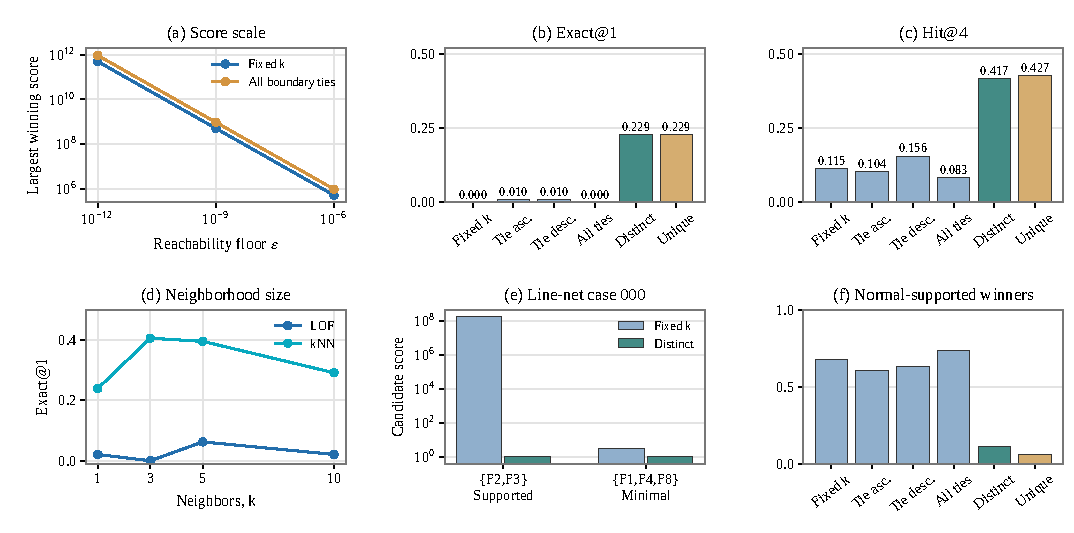
\includegraphics[width=\textwidth]{figures/figure_unified_lof.pdf}
\caption{Matched invoice LOF diagnostics, all 96 targets and 255 candidates. (a)--(b) Recovery under fixed-$k$ tie choices, all boundary ties, distinct-coordinate radii retaining multiplicities, and unique projections. (c) Fraction of winners already supported by a normal reference. (d) Numerical-floor sensitivity. (e) Original neighbor-count sweep. (f) Supported and valid-minimal candidates in line-net case 000. Recovery panels use equal-relation means; variants retain their stated neighborhood semantics.}
\label{fig:lof}
\end{figure*}

\subsection{Floor, ties, and duplicate-aware variants}
\textbf{Numerical floor.} With the original neighbor routine, changing $\epsilon$ from $10^{-6}$ through $10^{-9}$ to $10^{-12}$ changes score magnitudes by approximately six orders but leaves all first choices unchanged. Exact@1 remains 0.000 and Hit@4 0.115. Inclusive-boundary neighborhoods likewise retain Exact@1 0.000 and Hit@4 0.083 throughout the sweep. The large score scale is floor-dependent; the observed failure is not removed by these floor choices.

\textbf{Boundary ties.} Canonical ascending and descending fixed-$k$ tie choices change 58 and 54 of 96 first sets relative to the original routine. Both reach Exact@1 0.010; their Hit@4 values are 0.104 and 0.156. Including every $k$-distance boundary tie changes 54 first choices, but exact recovery remains zero. Thus, discrete ties materially affect which explanations are returned, while boundary inclusion alone does not resolve this reversal. The original fixed-$k$ implementation must remain distinguished from the original LOF neighborhood definition.

\textbf{Duplicate treatment.} A distinct-coordinate radius retaining reference multiplicities reaches Exact@1/Hit@4 of 0.229/0.417. Collapsing identical projections and using inclusive boundaries reaches 0.229/0.427. Their fractions of normal-supported winners fall to 0.115 and 0.063, versus 0.677 for the original routine. The variants change neighborhood semantics, and projection collapse also changes empirical weights. Both improve recovery but remain below kNN's Exact@1 0.406 on this workload.

Earlier diagnostic restrictions remain separate: hidden-role-only search reaches LOF Exact@1 0.219; fixed-$k$ projection deduplication and exploratory reference-percentile calibration each reach 0.240. The oracle restriction uses hidden information, and reference-percentile scores share the fitted graph rather than an independent calibration sample. Their purpose is explanation of the original ranking, not selection of the best variant after observing test results. Taken together, the interventions locate the additional phenomenon in cross-projection competition among duplicate-sensitive scores.

\section{External Targets and Practical Scope}
\subsection{Public corrected-field inspection}
\begin{table*}[t]
\centering
\caption{Public corrected-field inspection, mean $\pm$ SD. Source columns use 24 case scores; aggregate columns use three source means. Schema fixes singleton JSON decoding. Recall@3 covers recorded corrections. Inspections gives the first corrected field position within four suggestions; failure receives $d+1$ (6/9/10 fields). Retrieval failures score zero. Uniform entries describe analytic expectations and their heterogeneity. Bold and underlining mark the best and second-best means (lower for Inspections); ties share marks.}
\begin{tabular*}{\textwidth}{@{\extracolsep{\fill}}|l|rrr|rrrr|}
\hline
Method & \multicolumn{3}{c|}{FieldHit@1 by source (24 each)} & \multicolumn{4}{c|}{Equal-source mean (72)} \\
\cline{2-8}
 & Flights & Beers & Rayyan & FieldHit@1 & FieldHit@3 & Recall@3 & Inspections ($\downarrow$) \\
\hline
Qwen & $0.000\pm0.000$ & $0.125\pm0.338$ & $\underline{0.250\pm0.442}$ & $0.125\pm0.125$ & $0.139\pm0.146$ & $0.098\pm0.088$ & $8.000\pm0.944$ \\
Qwen (schema) & $\textbf{0.667}\pm\textbf{0.482}$ & $\underline{0.958\pm0.204}$ & $\textbf{0.333}\pm\textbf{0.482}$ & $\textbf{0.653}\pm\textbf{0.313}$ & $\textbf{0.833}\pm\textbf{0.253}$ & $\textbf{0.721}\pm\textbf{0.335}$ & $\textbf{2.819}\pm\textbf{2.651}$ \\
DeepSeek & $0.250\pm0.442$ & $0.083\pm0.282$ & $0.125\pm0.338$ & $0.153\pm0.087$ & $0.389\pm0.168$ & $0.286\pm0.162$ & $6.236\pm2.215$ \\
DeepSeek (schema) & $0.250\pm0.442$ & $0.083\pm0.282$ & $0.167\pm0.381$ & $0.167\pm0.083$ & $0.403\pm0.173$ & $0.291\pm0.163$ & $6.097\pm2.160$ \\
Llama & $0.042\pm0.204$ & $0.042\pm0.204$ & $0.083\pm0.282$ & $0.056\pm0.024$ & $0.153\pm0.105$ & $0.108\pm0.061$ & $8.028\pm1.850$ \\
Llama (schema) & $0.208\pm0.415$ & $0.750\pm0.442$ & $\underline{0.250\pm0.442}$ & $\underline{0.403\pm0.301}$ & $\underline{0.750\pm0.144}$ & $\underline{0.578\pm0.189}$ & $\underline{3.181\pm1.646}$ \\
Gower-LOF & $0.000\pm0.000$ & $\textbf{1.000}\pm\textbf{0.000}$ & $0.208\pm0.415$ & $\underline{0.403\pm0.528}$ & $0.597\pm0.364$ & $0.388\pm0.383$ & $3.750\pm2.567$ \\
Gower-kNN & $0.042\pm0.204$ & $\textbf{1.000}\pm\textbf{0.000}$ & $0.167\pm0.381$ & $\underline{0.403\pm0.521}$ & $0.708\pm0.260$ & $0.465\pm0.319$ & $3.681\pm2.730$ \\
Uniform (expected) & $\underline{0.361\pm0.182}$ & $0.227\pm0.101$ & $0.208\pm0.097$ & $0.265\pm0.083$ & $0.616\pm0.125$ & $0.378\pm0.107$ & $4.253\pm1.408$ \\
\hline
\end{tabular*}
\label{tab:real-cells}
\end{table*}

\begin{figure}[t]
\centering
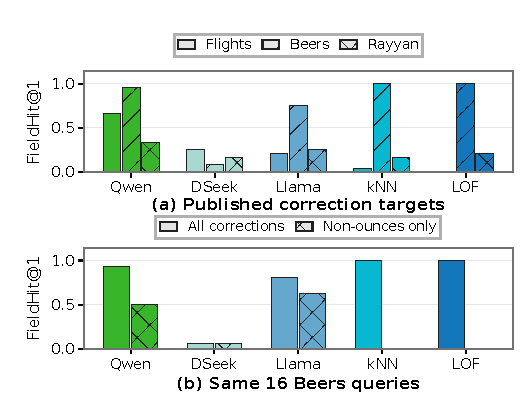
\includegraphics[width=\columnwidth]{figures/figure_unified_corrections.pdf}
\caption{Structured singleton inspection on published corrections. (a) Each source contains 24 targets. (b) The same 16 Beers queries with non-ounces corrections are evaluated against all recorded changes and then only non-ounces changes, with predictions fixed. These endpoints assess correction localization, not population-minimal support.}
\label{fig:corrections}
\end{figure}

Table~\ref{tab:real-cells} reports the original public-correction task and its fixed-schema condition. Fixed structured decoding raises Qwen's equal-source FieldHit@1 from 0.125 to 0.653, and Llama's from 0.056 to 0.403; both Gower controls score 0.403. Qwen covers 0.721 of recorded corrections within three suggestions. Its mean first-correction inspection score is 2.819, compared with kNN's 3.681 and an analytic uniform ordering's 4.253 under the same cap and failure penalty. These are offline ranking quantities, not measurements of analyst time.

\textbf{Correction type matters.} All 24 Beers targets contain an ounces representation change, and both Gower methods choose a corrected field first in every case. Our source audit identifies 24 quantity representations, 12 missing-marker normalizations, six city/state split changes, and seven percentage conventions. Seventeen rows contain only the explicitly checked row-local normalizations; seven mix them with percentage interpretation. Removing ounces from the accepted fields on the same 16 multi-correction queries reduces Gower FieldHit@1 to 0.000. Qwen and Llama retain 0.500 and 0.625; Gower Hit@3 remains 0.750. The first-choice result therefore depends strongly on the repeated ounces pattern, while later candidates retain useful coverage.

Flights contains 28 changed clock values and 21 imputations, alongside three clock-preserving format changes. The references exclude the query's flight; an actual-departure correction such as 11:06 to 11:05 requires event-specific evidence unavailable in other flights. Qwen's FieldHit@1 of 0.667 indicates selection of a recorded changed field, not recovery of that external fact. Rayyan contains date serialization, encoding normalization, missing sentinels, and other bibliographic conventions. The audit preserves those supplied labels without claiming an independent judgment that each canonical value is semantically correct. Neither source-convention agreement nor model consensus certifies a minimal explanation.

\begin{table*}[t]
\centering
\caption{Neighboring evaluation targets. Checkmarks denote primary targets, not exhaustive software capabilities. ``Fault'' includes integrity errors and injected faults; ``Support'' means population-minimal descriptive support.}
\begin{tabularx}{\textwidth}{|c|>{\raggedright\arraybackslash}p{1.75cm}|>{\raggedright\arraybackslash}X|c|c|c|c|c|c|}
\hline
\multirow{2}{*}{Category} & \multirow{2}{*}{Task / idea} & \multirow{2}{*}{Representative work} & \multicolumn{6}{c|}{Primary object of evaluation or explanation} \\
\cline{4-9}
 & & & Row & Score & Subspace & Group & Fault & Support \\
\hline
Model & Score attribution & Shapley explanation; CAIT~\cite{kluttermann2024shapley,mok2025cait} & -- & $\checkmark$ & -- & -- & -- & -- \\
\hline
\multirow{5}{*}{Data} & Subspace analysis & LookOut, SOD, COP~\cite{gupta2018lookout,kriegel2009sod} & -- & -- & $\checkmark$ & -- & -- & -- \\
\cline{2-9}
 & Field choices and repair mask & M\textsuperscript{2}OE~\cite{angiulli2024m2oe} & -- & -- & $\checkmark$ & -- & -- & -- \\
\cline{2-9}
 & Ranked subspace search & RLAX~\cite{amirato2026rlax} & -- & -- & $\checkmark$ & -- & -- & -- \\
\cline{2-9}
 & Aggregate diagnosis & Adtributor, iDice, HotSpot, Squeeze~\cite{bhagwan2014adtributor,lin2016idice,sun2018hotspot,li2019squeeze} & -- & -- & -- & $\checkmark$ & -- & -- \\
\cline{2-9}
 & Data cleaning & HoloClean; AutoDCWorkflow~\cite{rekatsinas2017holoclean,li2025autodcworkflow} & -- & -- & -- & -- & $\checkmark$ & -- \\
\hline
\multirow{4}{*}{Evaluation} & Anomaly benchmarks & ADBench, TABARD, RADAR~\cite{han2022adbench,choudhury2025tabard,gu2025radar} & $\checkmark$ & -- & -- & -- & $\checkmark$ & -- \\
\cline{2-9}
 & Relevant-subspace evaluation & Myrtakis et al.: Beam, RefOut, LookOut, HiCS~\cite{myrtakis2021comparative} & -- & -- & $\checkmark$ & -- & -- & -- \\
\cline{2-9}
 & Fault-label studies & Gate-negation circuit explanations~\cite{antwarg2024groundtruth} & -- & -- & $\checkmark$ & -- & $\checkmark$ & -- \\
\cline{2-9}
 & Minimal-set benchmark & This study: known outlier + finite references & -- & -- & $\checkmark$ & -- & -- & $\checkmark$ \\
\hline
\end{tabularx}
\label{tab:related-work}
\end{table*}

\subsection{Auxiliary pilots and interpretation}
The peer pilot retains 390 model outputs, including 349 valid non-abstentions. Pairwise Jaccard ranges from 0.213 to 0.520 on 40 ADBench queries answered by all five models; UCI has only one common-valid query. The archived Pima example in Fig.~\ref{fig:intro-real} has Qwen/peer-majority overlap 0.500, with no field-level truth. These measurements characterize agreement only.

With all circuit outputs visible, Qwen/DeepSeek/Llama achieve Jaccard@4 of 0.349/0.109/0.038, compared with input-only Gower-kNN/LOF at 0.456/0.428. Qwen's Hit@4 is 0.016 and the others retrieve no exact fault set. Scores average queries within targets, targets within table pairs, and pairs within four circuits. These fault labels and the limited number of circuits prevent treating the pilot as validation of population-minimal support.

\textbf{Method selection.} Specify whether the target is an irreducible combination, a rule mechanism, or a corrected field. For support, compare candidate coverage with rank: SME's first choice can be a spurious small set. For density search, inspect duplicates, ties, and score scales. For LLMs, evaluate the prompt, candidate information, decoder, parser, and abstention rule together. Rankings remain workload- and target-specific.

\textbf{Continuous and noisy data.} Independently sampled continuous values almost surely lack exact matches in finite references, making ordinary singletons appear explanatory. Extension requires a support model or explicit scales, tolerance neighborhoods, and a mass threshold; these change the gold labels. Finite invoice and expert domains avoid this ambiguity. Native continuous controls do not validate continuous support labels.

\section{Related Work}
Table~\ref{tab:related-work} compares the primary evaluation targets of neighboring work.

\textbf{Closest evaluation predecessor.} Myrtakis et al.~\cite{myrtakis2021comparative} use multiple relevant subspaces and exact membership in Recall/MAP, including outliers mixed with normal points in lower-dimensional projections. Our contribution is complete population-minimum enumeration, finite-reference audits, and separate rule/edit labels, rather than multiple answers or exact matching. Beam allows varying dimensionality; RefOut fixes it. A size-matched exhaustive control accompanies our Beam adaptation.



\textbf{Explanation objectives.} Surveys distinguish instance descriptions and detector-score explanations~\cite{panjei2022survey,li2024xadsurvey}. Shapley explanations and CAIT attribute model behavior~\cite{kluttermann2024shapley,mok2025cait}; LookOut, SOD, COP, and RLAX select subspaces~\cite{gupta2018lookout,kriegel2009sod,amirato2026rlax}. M\textsuperscript{2}OE also optimizes repairs~\cite{angiulli2024m2oe}. Scorpion, Adtributor, iDice, HotSpot, and Squeeze diagnose aggregate changes~\cite{wu2013scorpion,bhagwan2014adtributor,lin2016idice,sun2018hotspot,li2019squeeze}. Their targets can differ from support minima.

\textbf{Data quality and ICDE systems.} HoloClean, holistic repair, and AutoDCWorkflow address integrity errors~\cite{rekatsinas2017holoclean,chu2013holistic,li2025autodcworkflow}. BClean uses Bayesian networks and user priors~\cite{qin2024bclean}; ZeroED and ZeroEC use LLMs for detection and correction~\cite{ni2025zeroed,wu2025zeroec}. Query verification and AutoTest address further quality tasks~\cite{schreiber2026verification,chen2025autotest}. Our task withholds the clean target and evaluates field combinations.

\textbf{Benchmarks and component analysis.} ADBench benchmarks anomaly detection~\cite{han2022adbench}; TABARD, RADAR, AnTBench, and SEC-FinTables study perturbed tables, anomaly reasoning, awareness, and financial inconsistencies~\cite{choudhury2025tabard,gu2025radar,wei2026antbench,ke2026secfintables}. Papadakis et al.~\cite{papadakis2024reevaluation} examine candidate construction in record linkage. ICDE EAB studies decompose retrieval/generation, table retrieval, counting, and adaptive query processing~\cite{zhang2026xrag,yang2026tr360,zhu2026beacon,mu2026aqp}. We examine evidence, output contracts, and subspace ranking.

\section{Artifact and Reproducibility}
The public repository, \url{https://github.com/KDDElab/known-outlier-benchmark}, provides code, frozen inputs/labels/predictions, editable figures, manuscript sources, and environments. The README maps figures/tables to results and reconstruction commands. Provenance, licenses, model fingerprints, prompts, and decoding settings are recorded.

Archived checks cover population labels, Gower rankings, scalar LOF comparisons, and complete-population SME. Reconstruction from frozen outputs was checked on the original host; independent-machine and bitwise fresh-inference reproduction remain unverified.

\section{Conclusion and Limitations}
Population-minimal labels separate support, rules, and edits. Shared information and structured output support matched comparisons; enumeration separates coverage from ranking. Invoice reversal implicates projection duplicates and density-score competition. Corrections, circuit faults, and peer agreement remain distinct targets.

These conclusions concern three checkpoints and finite discrete domains. Templates overlap across seeds, earlier results informed protocol choices, and new rules were reused. Car largely admits singleton explanations; four invoice relations and four circuits limit coverage. Native checks do not establish convergence. Three reference draws and 24 complete-population targets cannot yield universal bounds; completeness also changes the prompt. Support--rule differences involve deterministic proxies; exact support does not directly extend to continuous noise. Temporal anomalies and MAR/MNAR missingness remain untested. Public corrections encode conventions, and expert decisions do not represent natural incidents. Human disagreement and time savings were not measured; pretraining exposure cannot be excluded, and fresh inference depends on software and checkpoint access.

\label{page:main-end}
\section*{Acknowledgments and AI Use Disclosure}
In the preparation of this paper, ChatGPT was used exclusively for the purpose of polishing and refining the linguistic style of certain sentences to improve readability and fluency in Sections I, III, and VII. All core intellectual contributions, including but not limited to:
\begin{itemize}
    \item \textbf{Original Ideas and Novel Viewpoints}: Any innovative concepts, hypotheses, and critical analysis are the product of the authors' own work.
\item \textbf{Experimental Data and Results}: All code, figures, findings, and interpretations thereof were generated, designed, collected, and analyzed by the authors.
\item \textbf{Substantive Descriptions of the Work}: The description of the methodology, experimental procedures, and discussion of the research implications were entirely authored by the research team.
\end{itemize}
\bibliographystyle{IEEEtran}
\bibliography{phase_d_references}
\end{document}
